\lecture{Randomized Minimum Cut}{Mon}{4}{Apr}{2016}

We consider the problem of computing the minimum number of edges we have to
remove from a graph such that it becomes disconnected.

\begin{definition}[Cut]
  Given a graph $G=(V,E)$, a \emph{cut} is a partitioning of the vertices into
  two nonempty sets $S$ and $V \setminus S$.
  The \emph{cut-set} of the cut is the set of edges between $S$ and
  $V \setminus S$, i.e., $(S \times (V \setminus S)) \cap E$.
  The \emph{size} of the cut is the cardinality of the cut-set.
\end{definition}

The \emph{minimum cut problem} is to find the size of the smallest
cut.\footnote{The algorithms we consider also compute a witness.}

\subsection{Karger's Algorithm}

The idea of the algorithm is based on the \emph{edge contraction} operation.
The contraction of an edge $\set{u,v}$ merges the nodes $u$ and $v$ into one,
retaining parallel edges but removing self-loops.
An example of edge contraction is given in Figure~\ref{fig:edge-contraction}.

\begin{figure}[h]
  \centering
  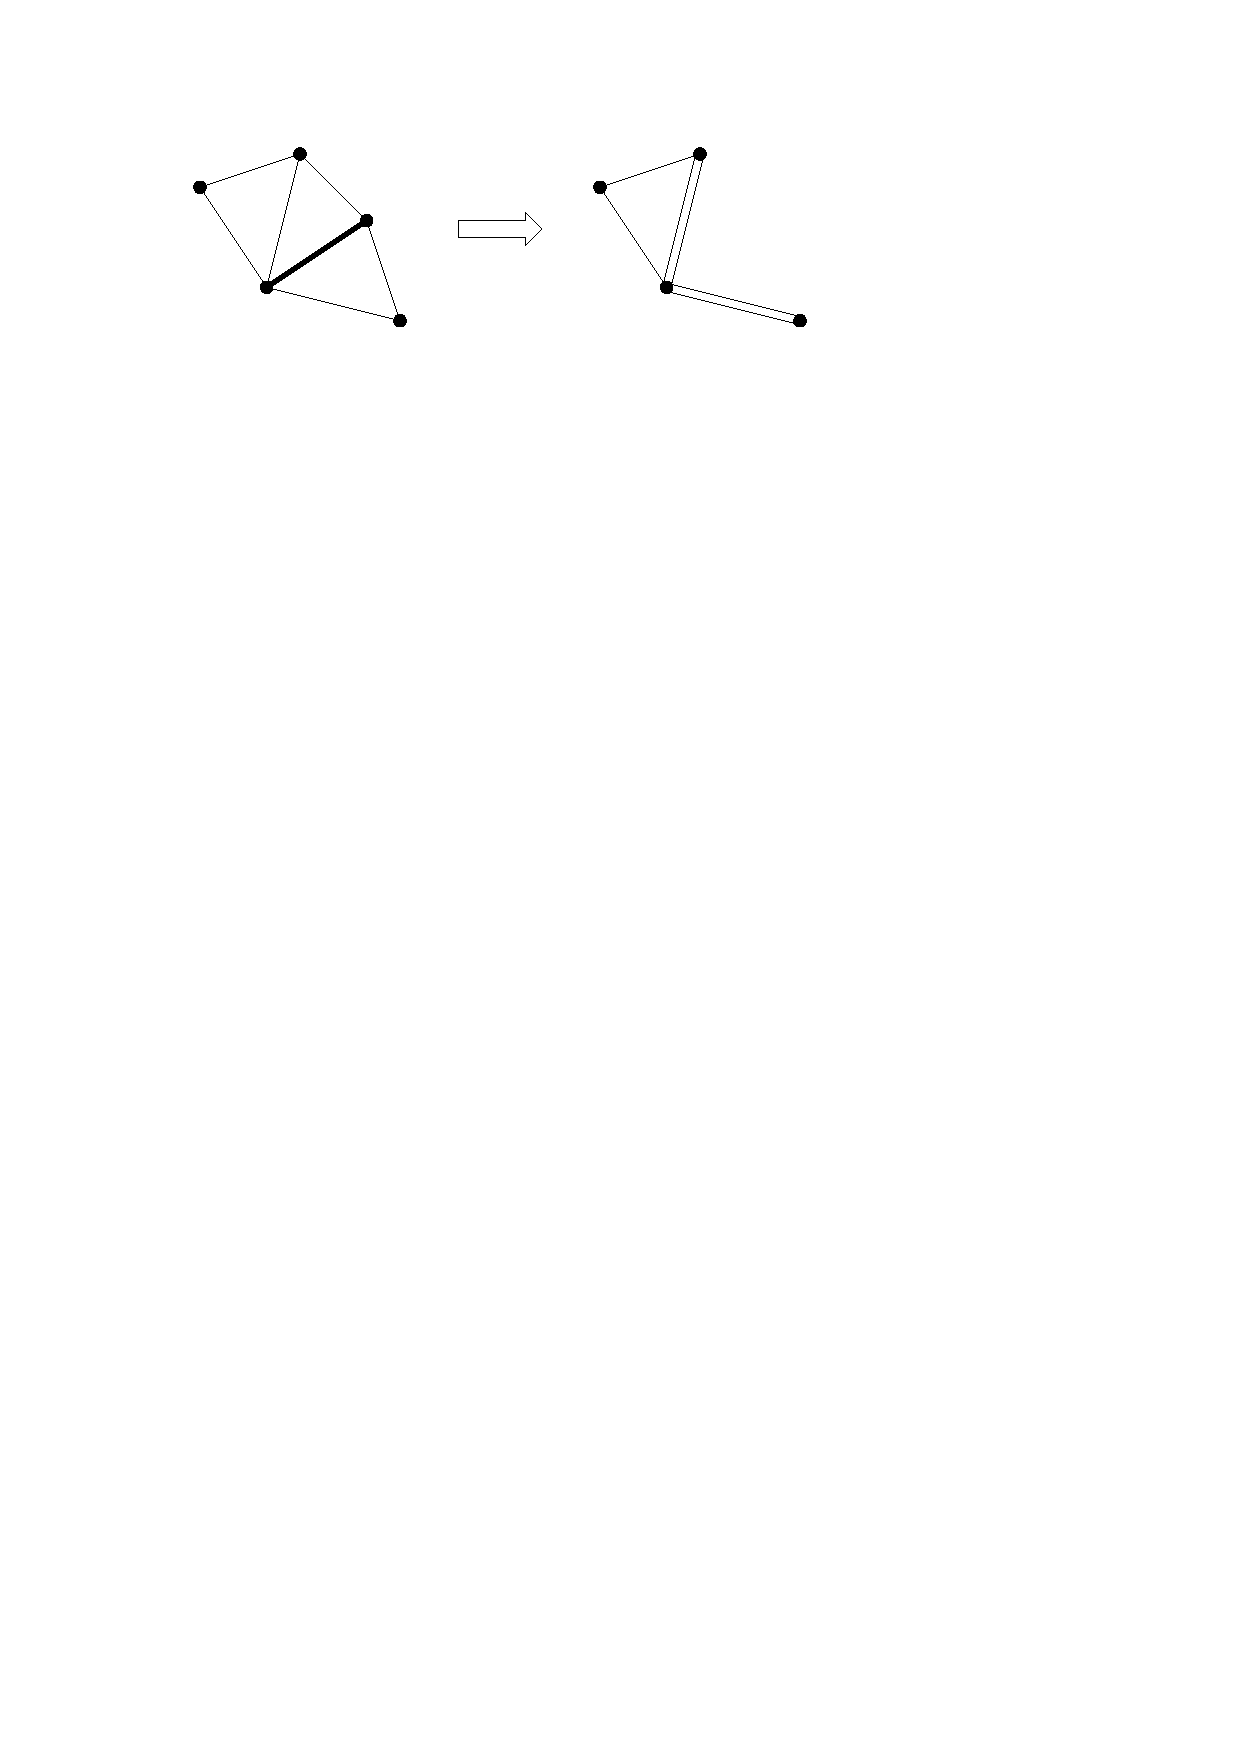
\includegraphics{edge-contraction}
  \caption{Result of contracting the thick edge.}
  \label{fig:edge-contraction}
\end{figure}

The contraction of an edge results in a multigraph with the number of nodes
reduced by one.
Karger's algorithm simply contracts randomly chosen edges until only two nodes
remain.

\begin{tabbing}
\hspace*{.25in} \= \hspace*{.25in} \= \hspace*{.25in} \= \hspace*{.25in} \= \hspace*{.25in} \=\kill
\>{\bf while} $|V| > 2$ \\
\>\> pick an edge $e \in E$ uniformly at random \\
\>\> contract $e$ \\
\>{\bf return} $|E|$
\end{tabbing}

It is easy to see that every cut in any intermediate graph corresponds to a cut
in the original graph.
However, the reverse is not true and thus the algorithm does not necessarily
find a minimum cut.
We will establish a bound on the success probability.
For the formal analysis let $n=|V|$ and $m=|E|$.
The presentation of the proof is taken from~\cite{MitzenmacherUpfal2005}.

\begin{theorem}
  Karger's algorithm outputs a minimum cut with probability at least $\frac{2}{n(n-1)}$.
\end{theorem}
\begin{proof}
  Let $k$ be the size of the min-cut set of $G$. 
  The graph may have several cut-sets of minimum size. 
  We compute the probability of finding one specific such set $C$.

  Since $C$ is a cut-set in the graph, removal of the set $C$ partitions the set
  of vertices into two sets, $S$ and $V \setminus S$, such that there are no
  edges connecting vertices in $S$ to vertices in $V \setminus S$. 
  Assume that, throughout an execution of the algorithm, we contract only edges
  that connect two vertices in $S$ or two vertices in $V \setminus S$, but not
  edges in $C$.
  In that case, all the edges eliminated throughout the execution will be edges
  connecting vertices in $S$ or vertices in $V \setminus S$, and after $n - 2$
  iterations the algorithm returns a graph with two vertices connected by the
  edges in $C$. 
  We may therefore conclude that, if the algorithm never chooses an edge of $C$
  in its $n - 2$ iterations, then the algorithm returns $C$ as the minimum
  cut-set.
  
  This argument gives some intuition for why we choose the edge at each
  iteration uniformly at random from the remaining existing edges. 
  If the size of the cut $C$ is small and if the algorithm chooses the edge
  uniformly at each step, then the probability that the algorithm chooses an
  edge of $C$ is small -- at least when the number of edges remaining is large
  compared to $C$.
  Let $E_i$ be the event that the edge contracted in iteration $i$ is not in
  $C$, and let $F_i = \bigcap_{j=1}^i E_j$ be the event that no edge of $C$ was
  contracted in the first $i$ iterations. 
  We need to compute $\Pr(F_{n-2})$.

  We start by computing $\Pr(E_1) = \Pr(F_1)$. 
  Since the minimum cut-set has $k$ edges, all vertices in the graph must have
  degree $k$ or larger. 
  If each vertex is adjacent to at least $k$ edges, then the graph must have at
  least $\frac{nk}{2}$ edges. 
  The first contracted edge is chosen uniformly at random from the set of all
  edges. 
  Since there are at least $\frac{nk}{2}$ edges in the graph and since $C$ has $k$ edges, the
  probability that we do not choose an edge of $C$ in the first iteration is given
  by
  \[\Pr(E_i) = \Pr(F_1) \geq 1 - \frac{2k}{nk} = 1 - \frac{2}{n}.\]

  Let us suppose that the first contraction did not eliminate an edge of $C$. 
  In other words, we condition on the event $F_1$. 
  Then, after the first iteration, we are left with an $(n - 1)$-node graph with
  minimum cut-set of size $k$. 
  Again, the degree of each vertex in the graph must be at least $k$, and the
  graph must have at least $\frac{k(n - 1)}{2}$ edges. 
  Thus,
  \[ \Pr(E_2 \mid F_1) \geq 1 - \frac{k}{k(n-1)/2} = 1 - \frac{2}{n-1}. \]
  Similarly,
  \[ \Pr(E_i \mid F_{i-1}) \geq 1 - \frac{k}{k(n-i+1)/2} = 1 - \frac{2}{n-i+1}. \]
  
  To compute $\Pr(F_{n-2})$, we use
  \begin{align*}
    \Pr(F_{n-2}) &= \Pr(E_{n-2} \cap F_{n-3}) = \Pr(E_{n-2} \mid F_{n-3}) \cdot \Pr(F_{n-3}) \\
                 &= \Pr(E_{n-2} \mid F_{n-3}) \cdot \Pr(E_{n-3} \mid F_{n-4}) \cdots \Pr(E_2 \mid F_1) \Pr(F_1) \\
                 &\geq \prod_{i=1}^{n-2} \left(1 - \frac{2}{n-i+1}\right) = \prod_{i=1}^{n-2} \left(\frac{n-i-1}{n-i+1}\right) \\
                 &= \left(\frac{n-2}{n}\right)\left(\frac{n-3}{n-1}\right)\left(\frac{n-4}{n-2}\right)
                   \cdots \left(\frac{4}{6}\right)\left(\frac{3}{5}\right)\left(\frac{2}{4}\right)\left(\frac{1}{3}\right) \\
                 &= \frac{2}{n(n-1)}.\qedhere
  \end{align*}
\end{proof}

Since the algorithm has a one-sided error, we can reduce the error probability
by repeating the algorithm. 
Assume that we run the randomized min-cut algorithm $n (n - 1) \ln n$ times and
output the minimum size cut-set found in all the iterations. 
The probability that the output is not a min-cut set is bounded by
\[ \left(1 - \frac{2}{n(n-1)}\right)^{n(n-1)\ln n} \leq e^{-2 \ln n} = \frac{1}{n^2}.\]
In the first inequality we have used the fact that $1-x \leq e^{-x}$.

However, every invocation of Karger's algorithm has running time $O(n^2)$, and
thus we end up with an $\widetilde{O}(n^4)$ algorithm. 
We will try to improve on that in the next section.

\subsection{Karger--Stein Algorithm}

Suppose we stop Karger's algorithm as soon as the graph was reduced to $t$ vertices.
The probability that a specific cut was avoided until this step is greater than
\[
\prod_{i=0}^{n-t-1} \left( 1 - \frac{2}{n-i} \right) = \frac {\binom{t}{2}}  {\binom{n}{2}},
\]
which becomes less than $\frac{1}{2}$ around $t = \frac{n}{\sqrt{2}}$.
Thus the idea of the Karger--Stein algorithm is to recursively contract two
copies of the input graph until this bound.


\begin{tabbing}
\hspace*{.25in} \= \hspace*{.25in} \= \hspace*{.25in} \= \hspace*{.25in} \= \hspace*{.25in} \=\kill
\>{\bf if} $|V| \leq 6$ (or some other small constant) \\
\>\> {\bf return} explicitly computed minimum cut \\
\>{\bf else} \\
\>\> obtain $G_1$ and $G_2$ by two independent runs of Karger's algorithm \\
\>\>\> until the graph has $\frac{|V|}{\sqrt{2}}$ vertices left\\
\>\> recurse on $G_1$ and $G_2$ \\
\>\> {\bf return} the minimum of both recursive calls
\end{tabbing}

The probability $P(n)$ that the algorithm finds a specific cut in an $n$-vertex
graph is given by the recurrence
\[
P(n) = 1 - \left( 1 - \frac{1}{2} P\left(\frac{n}{\sqrt{2}}\right)\right)^2.
\]

\begin{lemma}
  $P(n) \geq \frac{1}{\log n}$.
\end{lemma}
\begin{proof}
  By induction on $n$.
\end{proof}

The running time of the algorithm follows the recurrence
\[
T(n) = O(n^2) + 2 \cdot T\left(\frac{n}{\sqrt{2}}\right).
\]

\begin{lemma}
  $T(n) = O(n^2 \log n)$.
\end{lemma}
\begin{proof}
  By the master theorem.
\end{proof}

By repeating the algorithm $\log^2 n$ times, we obtain an error probability of
$\frac{1}{n}$ with an overall running time of $O(n^2 \log^3 n)$.

%%% Local Variables: 
%%% mode: latex
%%% TeX-master: "../main"
%%% End: 
